\documentclass[11pt]{article}
\usepackage{amssymb}
\usepackage{amsmath}
\usepackage{graphicx}
\usepackage{fullpage}
\usepackage{gensymb}
\usepackage{float}
\usepackage{upgreek}
\usepackage[]{hyperref}
\usepackage[margin=2cm]{geometry}
\tolerance=1000
\date{}
\title{Building Your Own Arduino}
\begin{document}
\maketitle

\centerline{
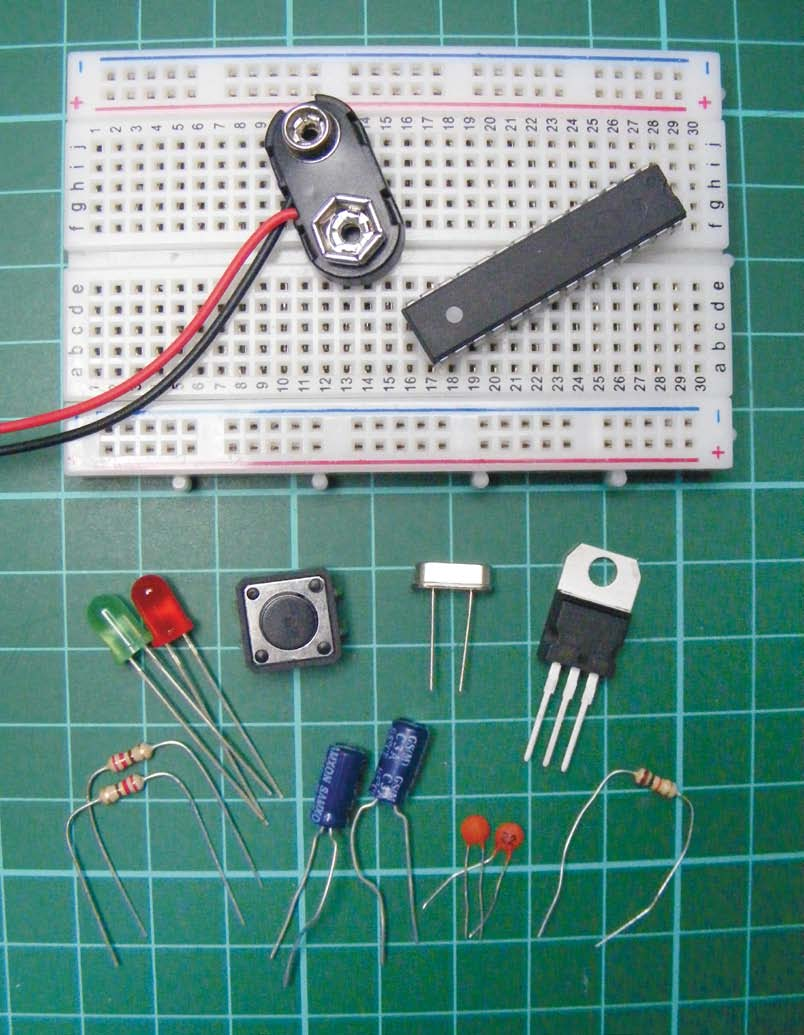
\includegraphics[scale=.55]{figures/cover.png}
}

\section{Setup}
Gather the required parts:

\begin{itemize}
  \begin{minipage}{0.4\linewidth}
         \item ATMEL ATmega328p chip
	 \item Breadboard
	 \item Green LED
	 \item Red LED
	 \item 3 220-ohm resistors
	 \item 16 MHz crystal oscillator (HC-495)
	 \item L7805cv 5V regulator
\end{minipage}
\begin{minipage}{0.4\linewidth}
  	 \item 2 100 $\mu$F electrolytic capacitors
	 \item PP3 9V battery clip
	 \item Momentary tactile four-pin pushbutton
	 \item 2 22 pF disc capacitors
	 \item Jumper wires
	 \item 9V battery
\end{minipage}
\end{itemize}

Here is an annotated version of the circuit you will be building to help you match
the part name to what the part looks like:

  \begin{figure}[htb]
    \centering
    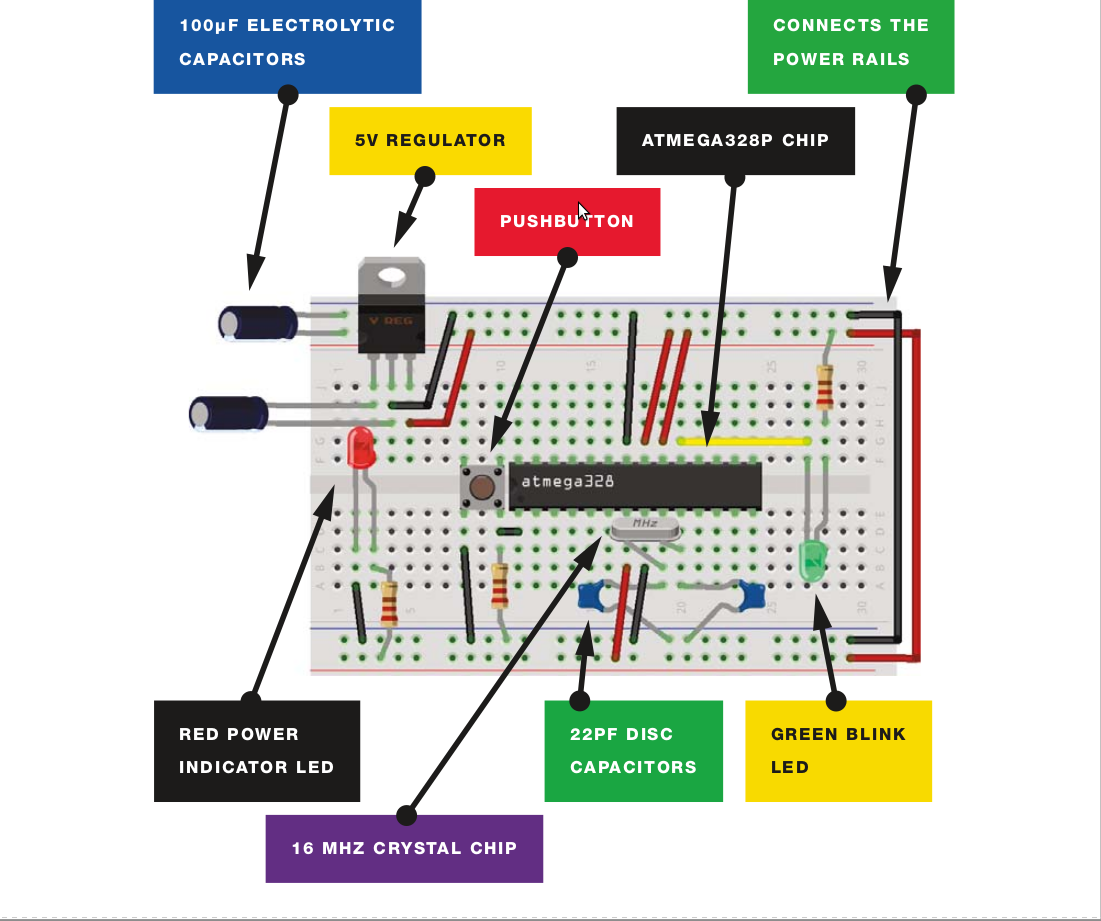
\includegraphics[width=.7\linewidth]{figures/schematic-annotated.png}
    \caption{\label{fig:schematic-annotated}}
  \end{figure}


\section{How it works}
\label{sec-2}
The custom Arduino is meant to be able to replicate the functionality of a Arduino
board. The custom board utilizes the ATMEL ATmega328p chip. This is the chip that
sits on the pre-built Ardunio boards we've been using (it is the brains of the
Arduino). It has some storage for programs onboard the chip, and must be programmed
via USB prior to using without the Arduino board just as we have been doing.

All of the parts listed above are found in every computer you encounter, from your
smartphone to your car, and are the essential components of what makes a computer
circuit from an electronics point of view. Here is what some of the stranger ones are
used for:

\begin{itemize}
\item {The 5V regulator limits the 9V battery to the 5V operating voltage of the
    ATmega chip (otherwise we risk burning out our chip!). Think of it like a mini
    surge protector + transformer like the ones you see on telephone poles.}
\item {The crystal oscillator is used to tell the Arduino how much time has past
    between one instant and the next (just like a clock). Inside the metal casing is
    a literal piece of quartz crystal that vibrates at a specific frequency when you
    run electricity through it, which the Arduino can then use.}
\item {The two types of capacitors are used to ensure that the ATMega input
    voltages/output signals chip are smooth and uninterrupted (i.e. reduces noise on
    input/output signals). What can happen is that there are temporary ``blips''
    (increases/decreases in voltage), which the capacitors help to smooth out. Think
    of what your furnace or air conditioning kicks on in your house/apartment---have
    you ever seen the lights momentarily flicker? That is a result of a larger
    version of one of these blips which are not harmful to things like lights, but
    definitely can be for sensitive electronics like the ATMega chip!}
\end{itemize}

Each ATmega328p chip has a tiny program permanently stored onboard that is
independent of the loaded sketches, called a \emph{bootloader} (think of it like the
BIOS on your computer). The bootloader's job is to actually load the sketches you
want to run into the chip's memory, just like the job of the BIOS is to load the
operating system you want to run (Windows, for example). Some ATMega328p chips come
preloaded with this bootloader, and sometimes you have to install it yourself! For
the chips we will be using, we already installed it for you.

The most important thing to remember when programming a custom Arduino is that you
need a Arduino board connected to a computer in order to load the sketch onto the
chip. The second most important thing is that the pinout of our custom Arduino
(i.e.~what pins do what) and that of the Arduino board are not the same, so you won't
be able to load sketches that you used successfully on an Arduino board onto our
custom board without modification. Fortunately, translating the pinouts is easy with
the aid of this handy table:

\begin{figure}[H]
  \centering
  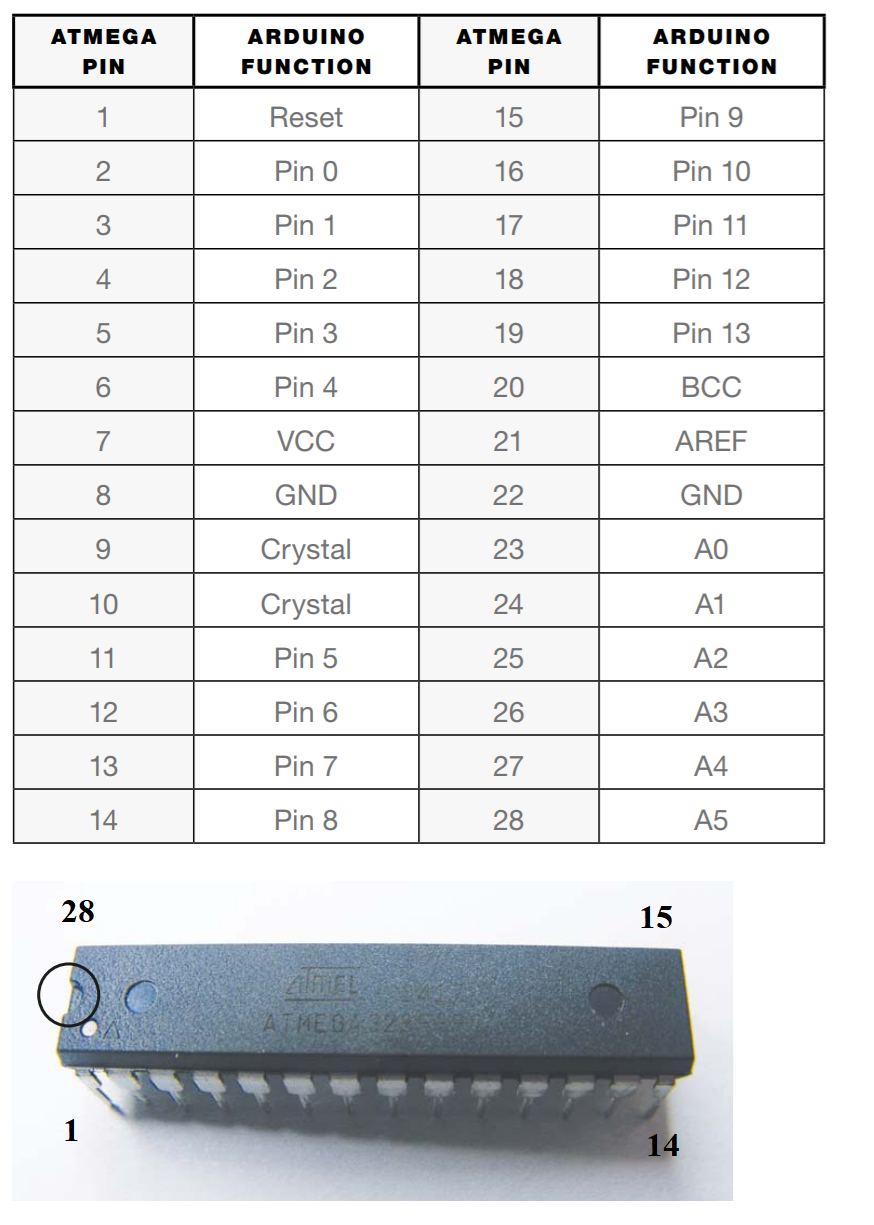
\includegraphics[width=.7\linewidth]{figures/atmega-pinout.png}
  \caption{\label{fig:atmega-pinoutput}}
\end{figure}

\section{Building The Circuit}
\label{sec-3}

Here is the final schematic for a fully functioning Arduino, so you see what we are
working towards:

\centerline{
  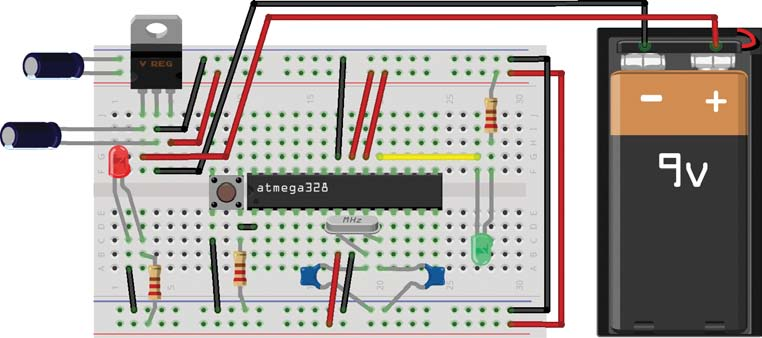
\includegraphics[width=.7\linewidth]{figures/build-6.png}
}

Surprisingly simple! Those components are all it takes to build a fully functioning
computer capable of running any of the programs we have seen so far.

For this circuit, for all the wires BUT the two connecting the power rails on each
side of the board and the two that go to the battery you should use small pieces of
wire that you cut and strip rather than the longer leads we have been using. This
will make it much easier to make your circuit, and much easier to attach various
additional hardware pieces to it!


\subsection{Import Things To Know When Building The Circuit}
{\bf IMPORTANT! READ THIS BEFORE STARTING}.

\begin{itemize}
\item {When building circuits on breadboards which holes are linked together matters a lot!
    Not all rows/columns of circuits are connected. See the diagrams below for an
    explanation of which holes are connected. The \emph{vertical} columns along the edges
    of the breadboard are connected, and the \emph{horizontal} rows in the middle part of
    the breadboard are connected. But, both the horizontal row and the vertical column
    connections do not cross the central line.

    \begin{figure}[H]
      \centering
      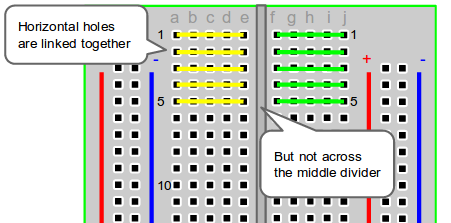
\includegraphics[width=\textwidth]{figures/breadboard-connectivity1.png}
      \caption{\label{fig:breadboard-connectivity1}}
    \end{figure}

    \begin{figure}[H]
      \centering
      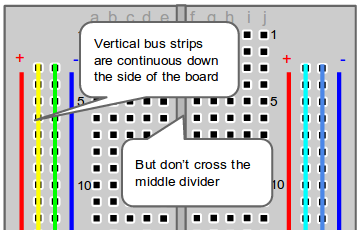
\includegraphics[width=\textwidth]{figures/breadboard-connectivity2.png}
      \caption{\label{fig:breadboard-connectivity2}}
    \end{figure}
  }
\item {When stripping wires for use on breadboards you generally want 0.25``'' at
    either end of the wire. Less and you risk the wire not making connection at both
    ends with the breadboard. More and the wire is probably too long for what you are
    doing.  }
  \item {It is a good idea to ask a volunteer/helper to verify your circuit is
      correct after each step, rather than waiting until the end. The problem is much
      easier to catch and figure out if there are less components on the breadboard.
    }
    \item {Use the same color wires as the diagram! It will make figuring out
        problems much easier. Or, you can choose to replace all red wires with blue,
        all yellow with green, etc.---just don't use random colors for all the
        wires. S13}
\end{itemize}

\subsection{Circuit Construction}
\begin{enumerate}
% \item {Connect the Arduino board to the PC and load the provided ``Blinking an LED''
%     sketch onto your ATmega chip on the Arduino board. You now have the brains of the
%     Arduino loaded with the sketch! Carefully pry the Arduino ATmega chip from your
%     existing Arduino board (Fig.~\ref{fig:build-0}), and begin assembling your custom
%     Arduino!}

%   \begin{figure}[H]
%     \centering
%     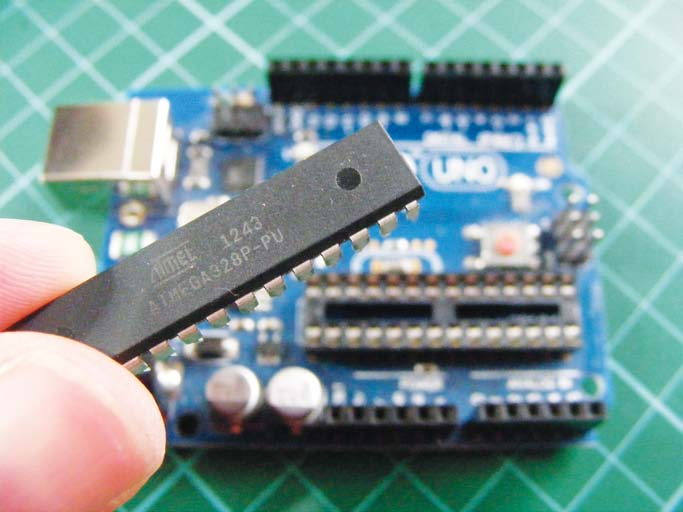
\includegraphics[width=.7\linewidth]{figures/build-0.png}
%     \caption{\label{fig:build-0}}
%   \end{figure}

\item {Insert the ATmega chip into the breadboard with its legs straddling
    either side of the center break. You need space at either end for components, so
    place it roughly as shown in Fig.~\ref{fig:build-1}.  Remember, pin 1 of the
    ATmega328p is directly below the small semicircle indentation on the chip. From
    here, pins are numbered 1--28 counterclockwise. Use this to position your chip
    correctly.  The semicircle should be on the \emph{LEFT} side of your circuit.}

  \begin{figure}[H]
    \centering
    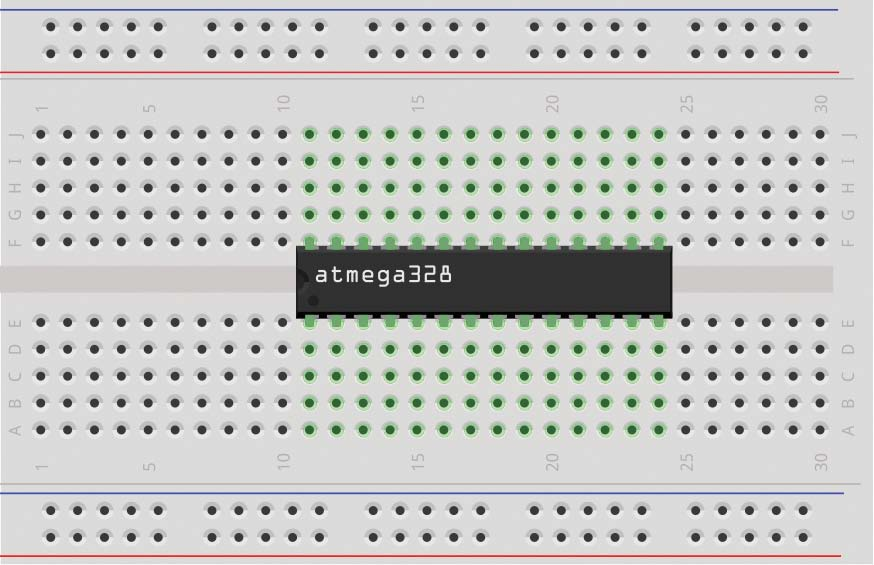
\includegraphics[width=.7\linewidth]{figures/build-1.png}
    \caption{\label{fig:build-1}}
  \end{figure}

\item {Connect pins 7, 20, and 21 of the ATmega to their closest positive power rail
    on the breadboard, and pins 8 and 23 to the negative power rails. Use jumper
    wires to connect the positive and GND power rails on either side of the board, as
    shown in Fig.~\ref{fig:build-2}.}

  \begin{figure}[H]
    \centering
    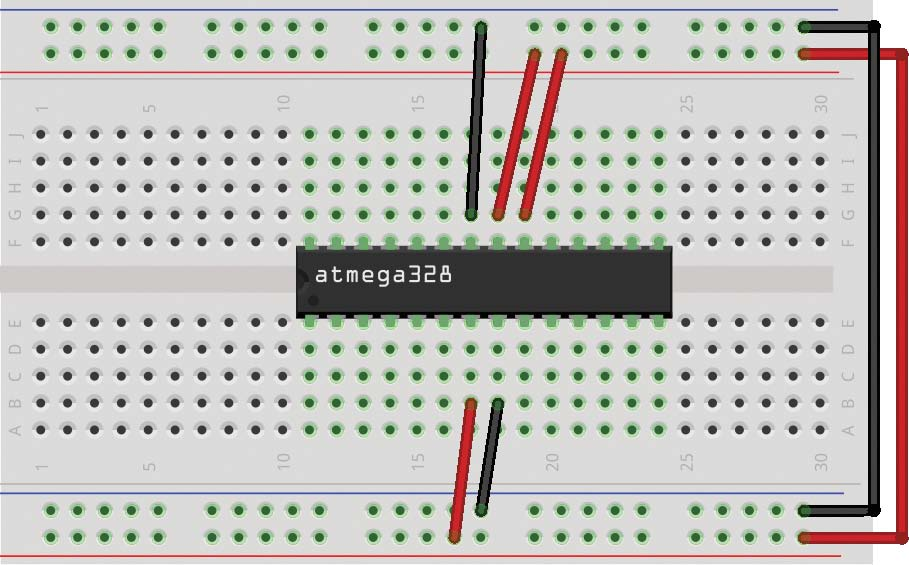
\includegraphics[width=.7\linewidth]{figures/build-2.png}
    \caption{\label{fig:build-2}}
  \end{figure}

\item {Connect one leg of the crystal oscillator to pin 9 on the ATmega chip, and
    connect the other leg to pin 10. Connect the legs of one of the 22 pF disc
    capacitors to pin 9 and GND, and the legs of the other disc capacitor to pin 10
    and GND, as shown in Figure~\ref{fig:build-3}.}

  \begin{figure}[H]
    \centering
    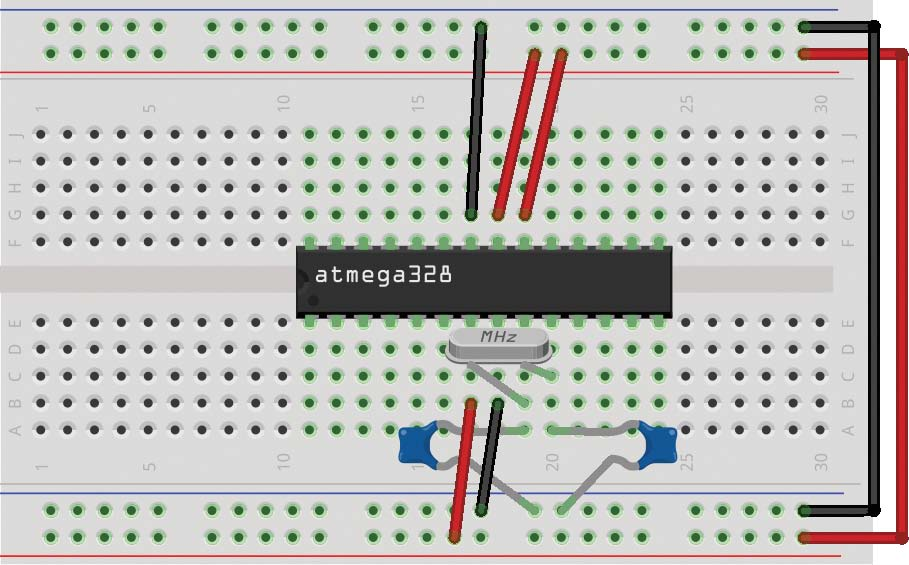
\includegraphics[width=.7\linewidth]{figures/build-3.png}
    \caption{\label{fig:build-3}}
  \end{figure}

\item {Insert the pushbutton into the breadboard to the left of the ATmega chip, with
    the legs straddling the center break in the breadboard. Using jumper wires,
    connect the lower-right pin of the pushbutton to pin 1 on the ATmega, and the
    lower-left pin to GND, as shown in Fig~ \ref{fig:build-4}. Connect a 220-ohm
    resistor to the lower-right pin, and connect the other side of this resistor to
    the {\bf POWER} rail (the diagram shows the {\bf GND} rail, which is
    incorrect). This pushbutton will act as our reset button.}

  \begin{figure}[H]
    \centering
    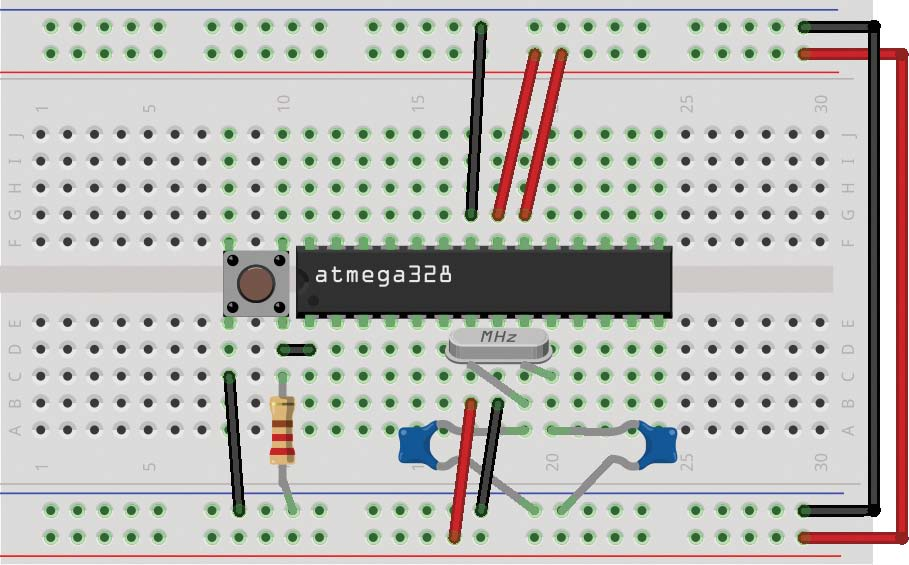
\includegraphics[width=.7\linewidth]{figures/build-4.png}
    \caption{\label{fig:build-4}}
  \end{figure}

\item {Insert the L7805cv 5V regulator into the top-left corner of the breadboard
    with the printed number of the component facing you, as shown in
    Fig.~\ref{fig:build-5}. The pins are numbered 1--3 from left to right. Insert one
    100 $\mu$F electrolytic capacitor into the top power rail of the breadboard, with
    one pin in the positive rail and the other pin in the negative rail. Connect the
    second 100$\mu$F electrolytic capacitor to pins 1 and 2 of the 5V regulator.
    Then connect pin 2 of the regulator to the negative power rail and pin 3 to the
    positive power rail.}

  \begin{figure}[H]
    \centering
    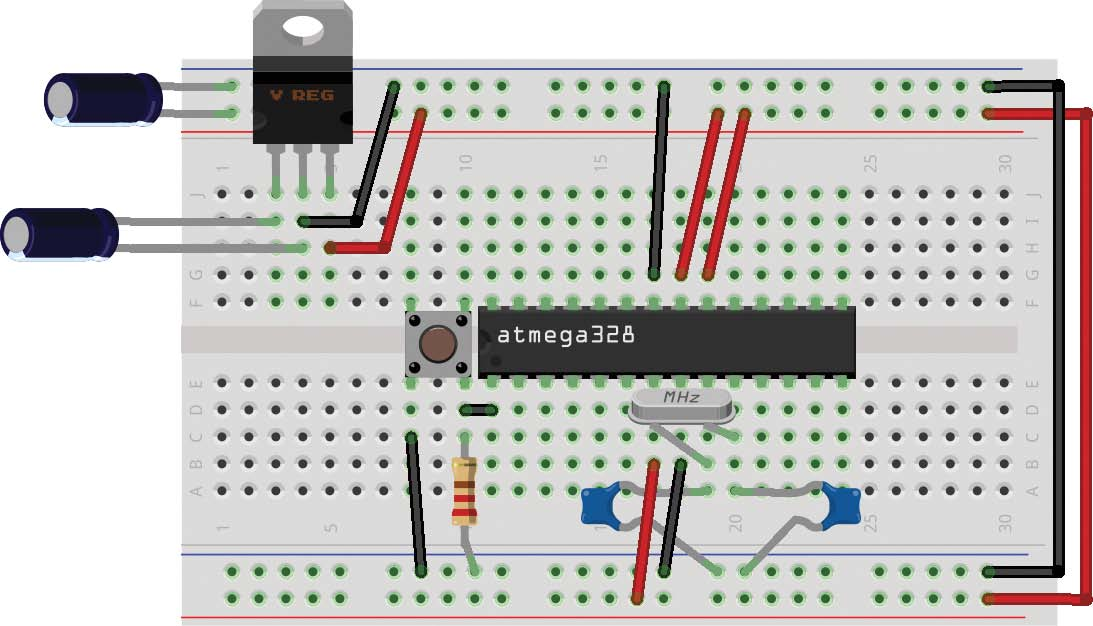
\includegraphics[width=.7\linewidth]{figures/build-5.png}
    \caption{\label{fig:build-5}}
  \end{figure}

\item {Insert the red LED into the breadboard, connecting the long, positive leg to
    the positive rail via a 220-ohm resistor, and the short, negative leg to
    GND. Then insert the green LED, connecting the short leg to pin 21 on the ATmega,
    and the long leg to the positive power rail via a 220-ohm resistor, as shown in
    Fig.~\ref{fig:build-6}. Add positive power from the battery to pin 1 on the 5V
    regulator and GND to pin 2 on the regulator.}

  \begin{figure}[H]
    \centering
    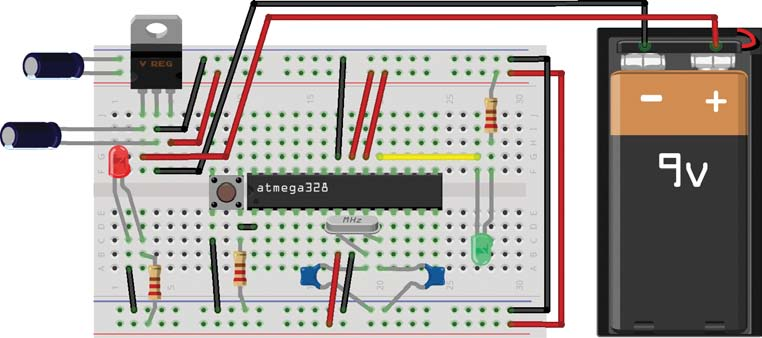
\includegraphics[width=.7\linewidth]{figures/build-6.png}
    \caption{\label{fig:build-6}}
  \end{figure}

\end{enumerate}

Your board is now complete and should look like Fig.~\ref{fig:build-6}.  The red LED
lights when power is added to the breadboard rails to indicate that the Arduino is on
and working, and the green LED lights in response to the ``Blinking an LED'' sketch
loaded on the ATmega chip (we loaded this for you ahead of time).


\section{The Code}
\label{sec-5}
A simple blinking LED code is provided to verify the functionality of the custom
built Arduino. This code uses pin 13 of the Arduino function and should make the
corresponding LED blink on the custom board.

\section{On Your Own}
\label{sec-6}
Now that the board's functionality is verified, the board is able to do anything that
a premade Arduino board can! The battery even allows the custom board to be used
without a connected computer, so you can actually do \emph{more} with this custom
board than you could with an Arduino board. The Arduino IDE comes preloaded with tons
of premade sketches that you can build the circuits for and load. See
\href{https://www.arduino.cc/en/Tutorial/BuiltInExamples}{https://www.arduino.cc/en/Tutorial/BuiltInExamples}
for descriptions of the sketches and the circuits.

Things to remember:

\begin{itemize}
\item You can't upload code to the DIY arduino directly. The easiest way to do this
  is with another Arduino board by removing the ATmega328P chip from the Arduino
  board and putting in the chip from your DIY Arduino (be careful not to bend the
  pins!), uploading the sketch to it, and then putting it back on your DIY Arduino
  breadboard. 
\item The pinout of the Arduino boards and the pinout of our custom Arduino are
  different, so be careful! Use the translation table in
  Fig.~\ref{fig:atmega-pinoutput} to make the necessary changes to the sketches you
  want to try.
\end{itemize}
\end{document}
